\documentclass[a4paper, 14pt]{report}
\usepackage[english, russian]{babel}
\usepackage[T2A]{fontenc}  % кодировка шрифта (кириллица)
\usepackage{graphicx}  % для работы с графикой
\graphicspath{{./images/}}
\usepackage[utf8]{inputenc}  % подключает UTF-8
\usepackage{setspace}  % интервалы
\onehalfspacing
\usepackage[left=30mm, top=20mm, right=10mm, bottom=20mm, nohead, footskip=10mm]{geometry}  % отступы
\usepackage[fontsize=14pt]{scrextend}  % размер текста
\usepackage[backend=biber,bibencoding=utf8,sorting=nty,maxcitenames=2,style=numeric-comp]{biblatex}  % список литературы
\addbibresource{bibliography.bib}

\begin{document}
	\chapter{Аппаратные средства вычислительной техники (АСВТ)}
	\section{Введение АСВТ}
	Аппаратные средства вычислительной техники являются одним из ключевых компонентов современных компьютеров. Рассмотрение этого предмета включает в себя описание основных компонентов компьютерной техники, таких как процессоры, оперативная память, жесткие диски, мониторы, клавиатуры и мыши.(\ref{cuda1})
	
	\begin{figure}[h]
		\centering
		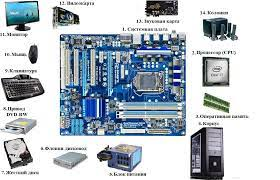
\includegraphics[scale=0.7]{cudaOne}
		\caption{Рассматриваемые компоненты}
		\label{cuda1}
	\end{figure}

	Формула для вычисления значения функции на элементах вектора X с использованием параллельного вычисления:(\ref{form1})
	
	\begin{equation}
		Y[i] = sin(X[i]) / cos(X[i])
		\label{form1}
	\end{equation}
	
	
	
	
	
\end{document}